\section{Measurement}
\label{section:measurement}

In this section we present the result of experiments, and discuss what we could deduct from these measurements. All the results we report here are from three or more runs, and only the plots from the most representative runs are shown. We drop all the page cache before doing each experiment, and during the experiment too when appropriate.

\subsection{Timer Calibration}
It is necessary to discuss how we measure times, since the accuracy of the timer we use is the basis of our measurement. We use the time stamp counter (tsc) and the rdtsc instruction on the x86 platform as our timer to guarantee the accuracy of our measurement. Since rdtsc returns clock counts instead of time, we write our own function to convert its result to second based on the CPU speed. This gives us up to nanosecond precision. However, since rdtsc is not synchronized across CPU, we may have problems using it in a multi-core machine. We cope with this by forcing our program to bind to one particular core and give it the highest priority to run until completion without context switch. To confirm the accuracy of our conversion, we in turn use our rdtsc function and gettimeofday() to measure the system call sleep(1) in 9 iterations in the non-virtualized/virtualized environment. 

\begin{table}[!thb]
\centering
\begin{tabular}{|c|c|c|} \hline
Iteration & rdtsc & gettimeofday \\ \hline
1 & 1.000126 & 1.000115 \\ \hline
2 & 1.000099 & 1.000088 \\ \hline
3 & 1.000099 & 1.000088 \\ \hline
4 & 1.000102 & 1.000091 \\ \hline
5 & 1.000098 & 1.000088 \\ \hline
6 & 1.000098 & 1.000087 \\ \hline
7 & 1.000100 & 1.000089 \\ \hline
8 & 1.000102 & 1.000093 \\ \hline
9 & 1.000109 & 1.000097 \\ \hline
\end{tabular}
\label{tab:cali_non_virtual}
\caption{Measuring sleep(1) in the non-virtualized environment}
\end{table}


\begin{table}[!thb]
\centering
\begin{tabular}{|c|c|c|} \hline
Iteration & rdtsc & gettimeofday \\ \hline
1 & 1.001859 & 1.002069 \\ \hline
2 & 1.000830 & 1.001039 \\ \hline
3 & 0.999983 & 1.000189 \\ \hline
4 & 1.000760 & 1.000967 \\ \hline
5 & 0.999982 & 1.000189 \\ \hline
6 & 1.001173 & 1.001388 \\ \hline
7 & 1.000029 & 1.000233 \\ \hline
8 & 1.000896 & 1.001109 \\ \hline
9 & 0.999955 & 1.000160 \\ \hline
\end{tabular}
\label{tab:cali_virtual}
\caption{Measuring sleep(1) in the virtualized environment}
\end{table}

The data in table 1 and 2 show that the results of rdtsc function and gettimeofday() are the same up to 3 significant decimals. It confirms that our rdtsc function has accuracy in 0.001 seconds or 1 microsecond.

\subsection{Ideal Buffer Size}
To find the ideal buffer size for random file access, we randomly access a large file with different buffer size, and measure how long it takes to read given size of data. Here we set the size of data to read is 32MB; and we vary buffer size from 512 bytes to 51200 bytes (0.5 KB - 50 KB). 

\begin{figure*}
\centering
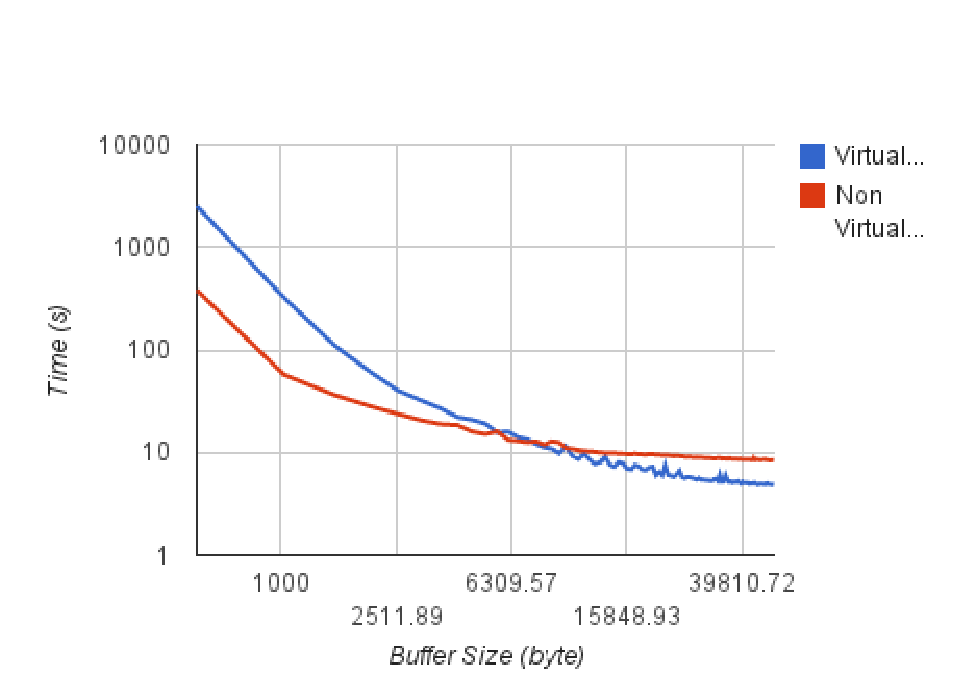
\includegraphics[width=.65\textwidth]{figures/buffer_size.eps}
\caption{Ideal Buffer Size Measurement}
\label{fig:buffer_size}
\end{figure*}

The measurement result is shown if figure \ref{fig:buffer_size}. In the non-virtualized setting, we could see that the time took to randomly read 32MB data decrease rapidly as the buffer size increase, until the buffer size is larger than 12KB, at which point the elapsed time start to stabilize. One would expect that any buffer size < 4KB would be suboptimal, since essentially a whole 4K block has to be read into memory even if you are filling a buffer which is much smaller than 4K. However, we do observe some additional performance gain further increasing the buffer size up to 12KB. This might be attributed to the fact that larger buffer size amortized the cost of initiating an I/O transfer from disk. But further experiments needs to be conducted to verify this hypothesis. 

Measurement results in the virtualized environment exhibited similar trends, where the reading time start to stabilize when the buffer size is larger than 20KB. However, there are two noticeable difference. First, with small buffer size, the random read performance is significantly worse than in a non-virtualized setting. This is expected because there is more overhead associated with each I/O in a virtual machine. Second, with larger buffer size, virtual machine actually outperforms a native operating system. This effect might be attributed to the fact that the host operating system memory served as a secondary level cache. However, more measurements are needed to confirm this guess. 

In summary, the idea buffer size is 12KB in non-virtualized setting, and 20KB in a virtualized setting.

\subsection{Prefetch Size}
In this experiment we are concerned about how much data is prefetched by the file system during a sequential read. In order to estimate this, we first open a file and read its first block; we then sleep for some time (40ms in our experiment) to allow the file system prefetching, finally we seek for a certain distance and read another block of this file. If this block is previously prefetched by the file system, then this read would be very fast; otherwise this read would be significantly slower. Thus by varying the distance of seeking, we would observe a jump of read latency at certain distance, and that would be the file system prefetch size. 

\begin{figure*}
\centering
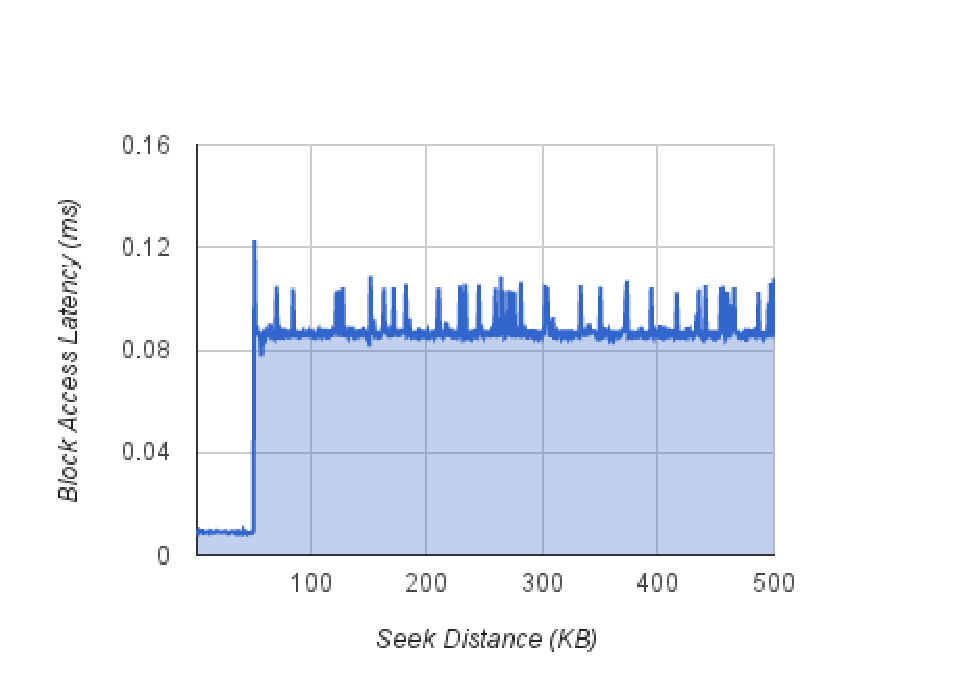
\includegraphics[width=.65\textwidth]{figures/prefetch_1.eps}
\caption{Prefetch Size Measurement in Non-virtualized Environment}
\label{fig:prefetch_1}
\end{figure*}

The measurement results in the non-virtualized setting are shown in figure \ref{fig:prefetch_1}. From the result we could see a clear jump at 50KB. Thus the prefetch size window of ext3 file system is most likely to be around 50KB.

\begin{figure*}
\centering
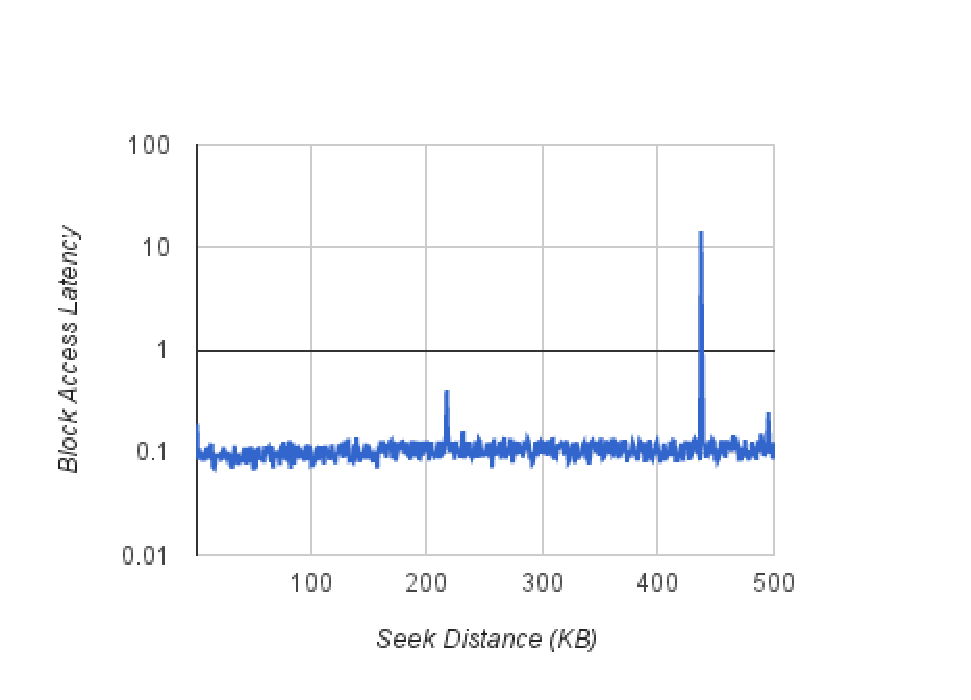
\includegraphics[width=.65\textwidth]{figures/prefetch_2.eps}
\caption{Prefetch Size Measurement in Virtualized Environment}
\label{fig:prefetch_2}
\end{figure*}

The measurement results in the virtualized setting, shown in figure \ref{fig:prefetch_2}, however, is more complicated. Instead of a simple staircase behavior, we observe occasionally spike in latency time. This is due to the fact that under VMWare workstation 9.0, the virtual disk is realized using files on the host file system. Thus when we access the virtual disk, the host file system will perform its own prefetching, in addition to the prefetching going on in the guest file system. This double prefetching causes most file block access being served from memory cache of either the guest or the host file system. However, occasionally the block we want to access is in neither system's cache, and the overhead of accessing such a block is significantly higher, causing the spikes in latency time. Due to this double prefetching effect, it is hard to draw any firm conclusion on the prefetch size. But we could be confident that it would be smaller than 437K, where we observe the spike. 


\subsection{File Cache Size}
In order to measure how big the file cache is, we repeatedly read a group of blocks. The rational behind this is repeated reads of a group of blocks will be very fast; but if the read size exceeds the cache size, performance will start to degrade due to paging effect.

\begin{figure*}
\centering
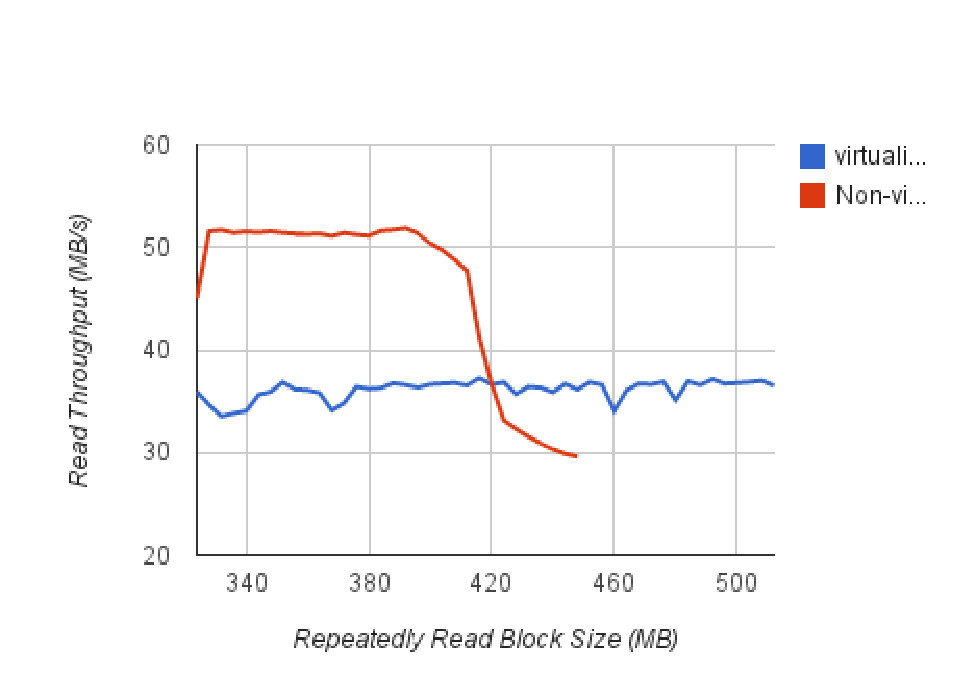
\includegraphics[width=.65\textwidth]{figures/cache_size.eps}
\caption{File Cache Size Measurement}
\label{fig:cache_size}
\end{figure*}

The memory size of the system we are measuring is 512MB, and the unified cache mechanism makes the most of this memory available for file cache under low memory pressure. Thus we vary the block group size we read from 324MB to 512MB, and the measurement results are shown in figure \ref{fig:cache_size}. In the non-virtualized setting, we could see a clear performance degradation starting from read size of 392MB. Thus the file cache is most likely to be around 392MB. In a virtualized setting, however, we don't see any performance degradation up to 512MB,which is the memory size of the guest operating system. This is because the host of the virtual machine we test has a large amount of memory (32GB), and any paging which might happen in the guest operating system is served from the host memory, which is fast enough and doesn't cause noticeable performance degradation. So from this experiment we cannot draw any conclusion on the file cache size of the guest operating system.


\subsection{Inode Holding Size}
Usually a file system inode can only hold pointers to a few blocks, and after that additional blocks must be read off disk containing more pointers. In this experiment we are interested at how many pointers are held in the inode, thus could be directly accessed from the inode; versus other blocks which have to be accessed through one or more indirect blocks which hold the pointers to their locations.

Our first attempt is to extend an empty file by one block repeatedly, and the force the change to the disk using fsync(). The idea is that is a block's pointer is held in the inode, adding this block only occurs two writes: one to the inode block, the other one to the newly added data block. However, if a block's pointer has to be accessed through some kind of indirection, one would have to update or allocate the indirection block(s) too. So extending a file to the point where an indirection layer is needed would be significantly slower than the situation where indirection is not necessarily. However, the time of extending a file stays constant, regardless of whether indirection is involved. This is because ext3/4 is a journaling file system, and by calling fsync() we only cause the journal to be committed to disk instead of actually writing the blocks to the in-place location. Since journal committing is a sequential write, writing one more block doesn't cause significant performance difference.

We instead try to read a block of a file at different offset: if we are accessing a block which is directly pointed from the inode, only one block access is needed; however, if we are accessing a block which requires indirection, one has to follow the indirection chain to find the location of the block before accessing it, resulting in two or more block accesses. If we disable file cache and force all the access to go to disk, significant performance difference might be observed. 

\begin{figure*}
\centering
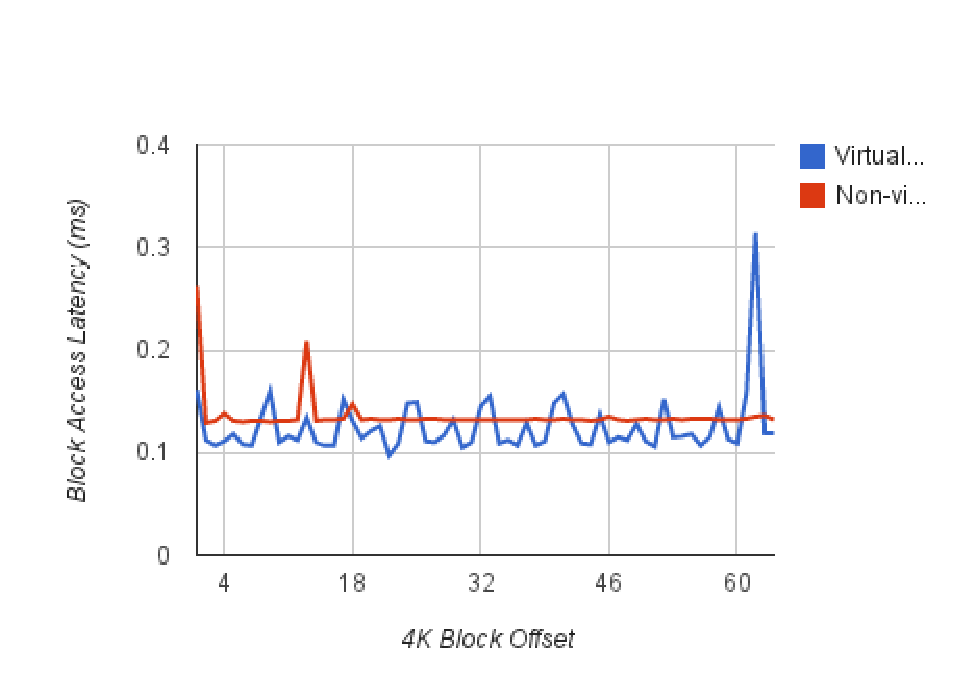
\includegraphics[width=.65\textwidth]{figures/indirect.eps}
\caption{Inode Holding Size Measurement}
\label{fig:indirect}
\end{figure*}

The measurement results are shown in figure \ref{fig:indirect}. For the non-virtualized setting results, we could easily see a spike at block offset 13, which is twice as much latency as accessing other blocks. This is due to the need to access one more indirect block. So we could conclude that in ext3, file system starts to add a layer of indirection when holding more than 12 blocks. The subsequent access to blocks after block 13 doesn't incur additional overhead because now the indirect information is cached in memory. The virtualized results are more difficult to understand though. Noticeably there is a spike at block offset 62, which could be caused by indirection. It is larger than the non-virtualized measurement because ext4 supports extent based addressing, which potentially allows inode to directly hold pointers to more blocks. However we could not exclude the possibility of this is the effect of some kind of paging happening in the host file system in order to access the virtual disk. We also see more fluctuation in the read latency, which is likely to be introduced by the complex guest/host interaction. However, it is hard to draw any conclusion on the inode holding size using this methodology in our virtualized setting. 
